\documentclass[12pt, onecolumn]{article}

\usepackage[utf8]{inputenc}
\usepackage[brazil]{babel}
\usepackage[top=2cm, bottom=2cm, right=2cm, left=2cm]{geometry}

\usepackage{graphicx}

\title{Matemática Discreta para Computação}
\author{Thiago Figueiredo Marcos}
\date{\today}

\begin{document}
	\maketitle
	
	\begin{abstract}
		
		Essa discplina será baseada na playlist Matemática Discreta
		(Fundamentos Matemáticos para Computação) disponível no youtube do canal 
		Prof. Douglas Maioli que tem uma vasta experiência em \texttt{educação}.
		Prof. Douglas tem Mestrado e Doutorado em Matemática Aplicada pela
		UNICAMP, além da Graduação em Licenciatura em Matematica pela UNESP. \\

		\textbf{Matematica Para Computação, Matematica Discreta}
	\end{abstract}

			%Introdução a Lógica Proposicional%
		%Aula - 1 Proposições, Tabelas verdades, conectivos%
		%Aula - 2 fbf, ordem de precedencia, Tauto e contradição %
		%Aula - 3 Equiva. e leis da eq. %
		%Aula - 4 Regras de inferência %
		%Aula - 5 Predicados e Quantificadores%
		%Aula - 6 Exemplos com prolog. %

		\section{\centering Introdução à Lógica Proposicional}

	Uma proposição é uma sentença que pode assumir valores \texttt{Verdadeiro} 
	ou \texttt{Falso}, não é necessário que se saiba o valor da sentença, apenas
	que seja possivel atribuir algum desses dois valores. \\
	\newline
	Sentenças que não são proposições, logicamente, não podem receber valores
	\texttt{Verdadeiros} ou \texttt{Falso}. Uma sentença declarativa que tenha 
	dependencia de variáveis pode ser considerada proposição, dês de que os 
	valores das variáveis sejam definidos. \\
	\newline
	Uma proposição segue três princípios:
	\begin{description}
		\item [\textbf{Príncipio da Identidade}]: 
			\texttt{"Uma proposição verdadeira é verdadeira 
			uma proposição falsa é falsa."}
		\item [\textbf{Príncipio da não-contradição}]: 
			\texttt{"Nenhuma proposição pode ser verdadeira e 
			falsa ao mesmo tempo."}
		\item [\textbf{Príncipio do terceiro-excluído}]: 
			\texttt{"Uma proposição ou será verdadeira ou será falsa:
			não há outra possibilidade."}
	\end{description}
	
		\subsection{Conectivos lógicos e Proposições Compostas}

	Conectivos lógicos podem ser entendidos como: \texttt{E}, \texttt{OU}, 
	\texttt{NÃO(NEGAÇÃO)}, \texttt{se ... então(IMPLICAÇÃO)}. Esses conectivos 
	permitem formar proposições compostas. \\
	\newline
	Uma proposição composta, possui na sua estrutura, composições simples ou 
	\texttt{atômica}. \\
	\newline
	\subsubsection{\centering Tabelas Verdade}
	Tabelas verdades são exemplificações gráficas das proposições e suas
	variáveis, conforme aumenta o número de variáveis aumenta o 
	número de combinaçõs, abaixo segue alguns exemplos: \\
	\begin{figure}[h]
		\centering
		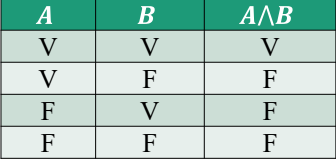
\includegraphics[width=0.3\textwidth]{./imagens/tabela-verdade-E.png}
		\caption{Conjunção}
		\label{fig:tab-e}
	\end{figure}
	
	\begin{figure}[h]
		\centering
		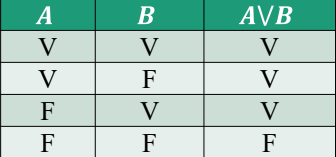
\includegraphics[width=0.3\textwidth]{./imagens/tabela-verdade-OU.png}
		\caption{Disjunção}
		\label{fig:tab-ou}
	\end{figure}

	\begin{figure}[h]
		\centering
		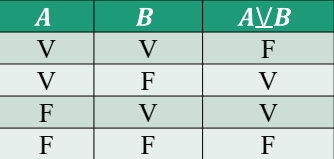
\includegraphics[width=0.3\textwidth]{./imagens/tabela-verdade-OUex.png}
		\caption{Disjunção Exclusiva}
		\label{fig:tab-ouex}
	\end{figure}

		\subsection{\centering Notação para cálculo proposicional}

	A lógica proposicional é um formalismo que nos permite determinar o valor 
	lógico das proposições. As letras minúsculas será a representação das 
	proposições. Abaixo descreveremos os sinais dos conectivos lógicos 
	\texttt{(operadores)}.\\
		\begin{description}
			\item[Conjunção]: $p \land q$
			\item[Disjunção]: $p \lor q$
			\item[Negação]: $\lnot p$ ou ainda $\bar{q}$
			\item[Condicional]: $p \Rightarrow q$
			\item[Bicondicional]: $p \Longleftrightarrow q$
			\item[Disjunção Exclusiva]: $p \oplus q$
		\end{description}

	A implicação é um dos mais importantes conectivos da lógica matemática. 
	Descreve-se da seguinte forma: 
	\begin{center}
		\texttt{Hipotese, premissa ou antecedente} \textbf{Verdadeira} 
		$\longrightarrow$
		\texttt{Tese, conclusão ou consequência} \textbf{verdadeira}
	\end{center}
		
		% Aula 2
	\subsection{\centering Procedência dos operadores lógicos}

	Em uma proposição que usa dois ou mais operadores lógicos a ordem em que são
	aplicados é importante. Podemos aplicar parenteses nas proposições para indicar
	a maior precedência. Também há regras para indicar a maior precedência entre
	os operadores: \\
	\\
		\begin{table}[h]
		\centering
			\begin{tabular}{|c|c|}
				\hline
				Operador & Precedência\\ \hline

				$\lnot$ & 1 \\
				$\land$ & 2 \\
				$\lor, \oplus$ & 3 \\
				$\Rightarrow, \Leftrightarrow$ & 4 \\
				\hline
			\end{tabular}
		\end{table}


	\subsection{\centering Tautologia e Contradições}
	
	Tautologia é uma proposição que é sempre verdadeira, para qualquer valor
	atômico que a componha, além disso uma cadeia que contenha uma expressão
	válida é denominada fórmula bem-formulada. \\
	\newline
	Pense na seguinte sentença: $P \lor \lnot P$, neste caso, \texttt{P}
	pode assumir qualquer valor que sua resposta será sempre verdadeira e
	isso é uma tautologia. Veremos como isso é aplicado diretamente na
	computação na disciplina de circuitos digitais em algebra boolena.\\
	\newline
	Já a contradição é uma proposição composta que é sempre falsa, para
	qualquer valor atômico que a componha.\\
	\newline
	Análogo a sentença da tautologia, porém com outro operador podemos
	exemplificar a contradição, observe: $P \land \lnot P$, ou seja, 
	p pode assumir qualquer valor, que sua proposição será sempre falsa.
	
	\subsection{\centering Equivalência Lógica ou Tautológica}

	Duas proposições são ditas equivalentes se possuirem valores lógicos iguais.
	Por exemplo: $P \Leftrightarrow \lnot(\lnot P)$ ou seja, operações
	com valores tautológicos, chegam a equivalências.\\
	\newline
	Para exemplificar ainda mais, se duas expressões com as mesmas variáveis
	assumirem os mesmos valores para operadores lógicos diferentes, essas duas
	expressões são \texttt{equivalentes}. 

	\subsubsection{\centering Leis de equivalência}
	
	\texttt{Leis do elemento identidade}:\\
	$P \land 1 \Rightarrow P$\\
	$P \lor 0 \Rightarrow P$\\
	$P \Leftrightarrow 1 \Rightarrow P$\\
	$P \oplus 0 \Rightarrow P$\\	
	\newline
	\texttt{Leis da idempotência}:\\
	$P \land P \Rightarrow P$\\
	$P \lor P \Rightarrow P$\\
	\newline
	\texttt{Leis da comutatividade}:\\
	$P \land Q \Rightarrow Q \land P$\\
	$P \lor Q \Rightarrow Q \lor P$\\
	$P \oplus Q \Rightarrow Q \oplus P$\\
	$P \Leftrightarrow Q \Rightarrow Q \Leftrightarrow P$\\
	\newline
	\texttt{Lei da redução ao absurdo}:\\
	$ -Q \Rightarrow Q \Rightarrow (P \land \lnot Q) \Rightarrow 0)$\\
	\newline
	Existem outras leis como a de \texttt{De Morgan} que vai ser vista com
	profundidade na disciplina de circuitos digitais e não será comentada aqui.
	Outras como associatividade e distributivas também não será vista, pois, 
	segue a mesma lógica que operações aritméticas.

			%% Aula 4
		\subsection{\centering Regras de Inferência}
	
	São regras de transformações de expressões que podem ser usadas
	para inferir uma conclusão a partir de premissas em forma de: 
	\begin{center}
		Hipótese $\Rightarrow$ Conclusão
	\end{center}
	Repare que a hipótese condiciona a uma conclusão, essa conclusão deve, 
	necessáriamente, ser verdadeira, para que a inferência, também seja. \\i
	Observe que na condicional a variável verdadeira, só poderá condicionar
	uma verdade, caso contrário a condicional é falsa. \\
	\newline
	Para deixar mais concreto, considere a seguinte sentença da banda 
	Charlie Brown Jr: \texttt{"Quem é de verdade sabe quem é de mentira"}
	na música \texttt{Pontes Indestrutíveis}. Aqui a variável verdadeira só
	pode condicinar verdades, do contrário, será falsa. 
	\newline
	A condicional é fundamental para se ter uma inferência, observe sua 
	tabela verdade:
	\begin{figure}[h]
		\centering
		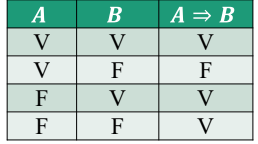
\includegraphics[width=0.3\textwidth]{./imagens/implicacao.png}
		\caption{Condicional}
		\label{fig:condicional}
	\end{figure}

	\begin{center}
		$(\lnot{A} \land B) \Rightarrow  (C)$
	\end{center}
	Essa inferência só vai ser falsa se, e somente se o lardo esquerdo da expressão,
	ou seja, $(\lnot{A} \land B)$ for verdadeiro e o lado direito da expressão, ou 
	seja C for falso. Este é o único caso em que a inferência é falsa, e pode 
	ser observado na tabela verdade da condicional. \\
	\newline
	Repare que, essas expressões, são um conjunto de combinações dos valores
	possíveis de cada variável, e determinada combinação para A, B e C fará com que
	a inferência seja falsa, e esses valores são respectivamente:
	\begin{center}
		$\lnot{A}$ = 1, B =  1, C = 0
	\end{center}
	Agora considere a seguinte sentença: 
	\begin{center}
		$((A \Rightarrow B) \land A) \Rightarrow B$
	\end{center}
	Neste caso, podemos análisar primeiramente a sentença interna 
	A $\Rightarrow$ B essa condicional só vai ser falsa se A for 
	verdadeira e B for falsa. \\
	\newline
	Agora temos o operador lógico $\land$ e a sentença do lado esquerdo da 
	inferência só vai ser falsa, se uma das variáveis for falsa. \\

	Aqui podemos observar o seguinte, o lado esquerdo da sentença só 
	vai ser verdadeiro se A e B forem verdadeiros ao mesmo tempo, isso
	quase que intuitivamente condiciona a sentença a uma verdade, essa
	estrutura é chamado de \texttt{Modus Ponens} ou \texttt{Mp.} \\
	\newline
	O seu inverso é chamado de \texttt{Modus Tollens} ou \texttt{Mt.}
	e pode ser observada do seguinte modo: 
	\begin{center}
		$((A \Rightarrow B) \land \lnot{B} \Rightarrow \lnot{A})$
	\end{center}
	%Aula 5
		\subsection{\centering Predicados e Quantificadores}
	
	A matemática discreta se concentra em estudar objetos discretos e pode
	ser aplicada aos mais diversos contextos da Biologia à Ciencias Sociais, ou
	seja, uma variável pode assumir diversos valores com base no seu conjunto
	universo, portanto, predicado é uma sentença em aberto, ou seja, 
	as variáveis que compoem a sentença precisa necessáriamente estar fora de 
	qualquer conjunto universo ou ainda, não se pode determinar o valor absoluto 
	da variável para se tornar uma proposição. \\

	Observe a seguinte sentença: \\ 
	\centering{$P(x) | x^2 < 9$}


\end{document}
